\subsection{The discrete element method with particle replacement}\label{sec:m-dem}

\emph{Theory and source.} A crusher sets the product, the throughput and the power through what happens to every rock in its chamber: the rock is
caught between a moving and a fixed surface, loaded, broken into progeny that fall and are caught again, until it leaves through the discharge gap.
The population balances of the preceding subsections describe this with a classification and a breakage function fitted to plant data. The
discrete element method follows each rock as a body of its own, integrates Newton's equations for it and for its contacts, and lets the product
emerge from the mechanism; it is the reference with which crusher models are compared in the literature~\cite{cleary2015,quist2016}. Two families
handle the breakage of a rock in such a simulation. A bonded-particle model builds each rock from many small spheres joined by bonds that fail; it
resolves cracks and is the most expensive: Quist reports $172$ and $404$ CPU hours for four seconds of a quarter section of an industrial cone
crusher with $50{,}364$ and $92{,}508$ particles~\cite{quist2012}. A particle-replacement model keeps each rock as one sphere, accumulates the
energy of its collisions and, when that energy passes the rock's fracture energy, removes the sphere and puts its progeny in its place; its cost is
that of the spheres alone and its parameters come from single-particle tests. The product implements the second family, with the single-particle
breakage model of Tavares~\cite{tavares2022}, because its progeny law is the $t_{10}$ family that the population balance of Section~\ref{sec:m-breakage}
already uses, because its ore parameters can be derived from single-particle tests, and because a complete worked application to a laboratory jaw
crusher with its machine, ore and measurements is published in open access~\cite{barrios2020}. The method is run by the separate package
\texttt{crushdem}~\cite{crushdem2026}, never by code of the product; the product consumes the package's case of that laboratory jaw
(\emph{Implementation}, below). Symbols are those of Table~\ref{tab:notation}; the subscripts $i$ and $j$ name spheres and $w$ a wall.

\emph{Equations of motion.} A sphere $i$ has mass $m_i$, radius $R_i$, position $\mathbf q_i$, velocity $\mathbf v_i$, spin $\boldsymbol\omega_i$ and moment
of inertia $I_i=\tfrac25 m_iR_i^2$. Its translation and rotation follow
\begin{equation}
m_i\dot{\mathbf v}_i = m_i\mathbf g + \sum_{j}\left(\mathbf F^{\mathrm n}_{ij}+\mathbf F^{\mathrm t}_{ij}\right) + \sum_{w}\left(\mathbf F^{\mathrm n}_{iw}+\mathbf F^{\mathrm t}_{iw}\right),\qquad
I_i\dot{\boldsymbol\omega}_i = \sum_{c} R_i\,\mathbf n_c\times\mathbf F^{\mathrm t}_c + \mathbf M^{\mathrm r}_i ,
\label{eq:dem-newton}
\end{equation}
with $\mathbf g$ the gravity (along $-z$), $\mathbf F^{\mathrm n}$ and $\mathbf F^{\mathrm t}$ the normal and tangential contact forces, $\mathbf n_c$ the
unit normal of contact $c$ and $\mathbf M^{\mathrm r}_i$ the rolling torque. Spheres may have any radius in an open three-dimensional domain; the domain has
no periodic boundary. A wall is a thin, two-sided analytic surface of infinite mass and stiffness; a sphere-wall contact uses the same contact law with
the wall as the second body (infinite radius and mass) and the wall's velocity at the contact point.

\emph{Contact kinematics.} Two spheres of Young's moduli $Y$, Poisson ratios $\nu_{\mathrm P}$, shear moduli $G_{\mathrm{sh}}=Y/[2(1+\nu_{\mathrm P})]$ and masses $m$ have the
effective quantities
\begin{equation}
Y^{\ast} = \left(\frac{1-\nu_{\mathrm P,i}^2}{Y_i}+\frac{1-\nu_{\mathrm P,j}^2}{Y_j}\right)^{-1},\quad
G^{\ast}_{\mathrm{sh}} = \left(\frac{2-\nu_{\mathrm P,i}}{G_{\mathrm{sh},i}}+\frac{2-\nu_{\mathrm P,j}}{G_{\mathrm{sh},j}}\right)^{-1},\quad
R^{\ast}=\frac{R_iR_j}{R_i+R_j},\quad m^{\ast}=\frac{m_im_j}{m_i+m_j},
\label{eq:dem-eff}
\end{equation}
and overlap by $\delta_{\mathrm c}=R_i+R_j-\lVert\mathbf q_j-\mathbf q_i\rVert$; the contact exists only for $\delta_{\mathrm c}>0$, so two spheres that touch
at zero overlap exert no force. For a contact with a wall, $m^{\ast}$ is the mass of the sphere. These are the quantities of the Hertz-Mindlin
contact as the documentation of the LAMMPS granular pair style states them~\cite{lammpsgranular}.

\emph{Normal force with the restitution damping.} The normal force is the Hertz elastic force plus a damper whose constant follows from the
coefficient of restitution $e_{\mathrm r}$ by the fit of Tsuji, Tanaka and Ishida~\cite{tsuji1992},
\begin{equation}
F^{\mathrm n} = \tfrac43\,Y^{\ast}\sqrt{R^{\ast}}\,\delta_{\mathrm c}^{3/2} + \eta_{\mathrm n} v_{\mathrm n},\qquad
\eta_{\mathrm n}=\alpha(e_{\mathrm r})\sqrt{m^{\ast}k_{\mathrm{nd}}},\quad k_{\mathrm{nd}}=\tfrac43\,Y^{\ast}\sqrt{R^{\ast}\delta_{\mathrm c}},
\label{eq:dem-hertz}
\end{equation}
\begin{equation}
\frac{\alpha(e_{\mathrm r})}{\sqrt2} = 1.2728 - 4.2783\,e_{\mathrm r} + 11.087\,e_{\mathrm r}^2 - 22.348\,e_{\mathrm r}^3 + 27.467\,e_{\mathrm r}^4 - 18.022\,e_{\mathrm r}^5 + 4.8218\,e_{\mathrm r}^6 ,
\label{eq:dem-tsuji}
\end{equation}
where $v_{\mathrm n}$ is the normal component of the relative velocity of the two contact points, positive while the spheres approach, so that the damper
resists both approach and separation. The constants of Equation~\eqref{eq:dem-tsuji} are read from the documentation of the LAMMPS style, as documented there (the constants of the original paper were not checked in this work); $\alpha(1)$ is set to zero exactly, because the polynomial leaves $4\times10^{-4}$ there and an
elastic contact must dissipate nothing. Because $\eta_{\mathrm n}$ grows as $\delta_{\mathrm c}^{1/4}$ the restitution does not depend on the impact speed. The
force is not clamped at zero: near the end of unloading the damper can exceed the spring and the force turns slightly attractive, as in the published
model. A clamp raises the restitution (a target of $0.2$ gave $0.325$ in a one-dimensional integration of the same law), while the unclamped law
reproduces the target to $0.002$; over $e_{\mathrm r}=0.2$ to $0.9$ and impact speeds of $0.05$ to $3$~m/s the largest error of the implementation is $0.0013$
(\texttt{test\_restitution\_is\_reproduced}, tolerance $0.005$).

\emph{Tangential force with history and Coulomb sliding.} The tangential force is a spring on the accumulated tangential displacement $\boldsymbol\xi$ of the
contact points, with a damper,
\begin{equation}
\boldsymbol\xi_{k+1} = \mathrm R_{\mathbf n}\,\boldsymbol\xi_k + \mathbf v_{\mathrm t}\,\Delta t,\qquad
k_{\mathrm t}=8\,G^{\ast}_{\mathrm{sh}}\sqrt{R^{\ast}\delta_{\mathrm c}},\qquad
\mathbf F^{\mathrm t}=-k_{\mathrm t}\boldsymbol\xi-\eta_{\mathrm t}\mathbf v_{\mathrm t},\quad \eta_{\mathrm t}=x_{\gamma,t}\,\eta_{\mathrm n},
\label{eq:dem-tangent}
\end{equation}
\begin{equation}
\text{if }\lVert\mathbf F^{\mathrm t}\rVert>\mu_{\mathrm c}\max(F^{\mathrm n},0):\quad
\mathbf F^{\mathrm t}\leftarrow\mu_{\mathrm c}\max(F^{\mathrm n},0)\frac{\mathbf F^{\mathrm t}}{\lVert\mathbf F^{\mathrm t}\rVert},\quad
\boldsymbol\xi\leftarrow-\frac{\mathbf F^{\mathrm t}+\eta_{\mathrm t}\mathbf v_{\mathrm t}}{k_{\mathrm t}} ,
\label{eq:dem-coulomb}
\end{equation}
with $\mathbf v_{\mathrm t}$ the tangential relative velocity of the contact points including the spins, $\mathrm R_{\mathbf n}$ the rotation that projects the spring onto the
current tangent plane while keeping its length, $\mu_{\mathrm c}$ the Coulomb coefficient and $x_{\gamma,t}$ the tangential damping ratio (one in the package, and in
the case). The history of a contact starts at zero when the contact begins and is dropped when it ends: each sphere stores, per contact partner, the spring
of the current step, and a partner absent from the neighbour list at the next step is forgotten. A wall contact is stored in the same table under the
wall's own identifier, so the spring survives between steps exactly as for two spheres. A constant directional torque opposes the relative spin of
a pair, $\mathbf M^{\mathrm r}_i=-\mu_{\mathrm r}R^{\ast}\max(F^{\mathrm n},0)\,\boldsymbol\omega_{\mathrm t}/\max(\lVert\boldsymbol\omega_{\mathrm t}\rVert,\omega_\epsilon)$, with $\boldsymbol\omega_{\mathrm t}$ the
relative spin of the pair projected on the tangent plane, $\mu_{\mathrm r}$ the rolling coefficient and $\omega_\epsilon=10^{-2}$~rad/s a regularisation that avoids the chatter of a sign
function at zero spin; this is the constant-torque category of the rolling-resistance models reviewed by Ai and co-workers~\cite{ai2011}, with the lever arm $R^{\ast}$ the choice of the package's
authors (the review was read for its model categories only). The laboratory-jaw case sets $\mu_{\mathrm r}$ from the paper's Table 4 (Table~\ref{tab:dem-params}).

\emph{Integration and the time step.} Velocity Verlet in kick-drift-kick form advances the state at a fixed step $\Delta t$,
\begin{equation}
\mathbf v\leftarrow\mathbf v+\tfrac{\Delta t}{2}\mathbf a,\quad\mathbf q\leftarrow\mathbf q+\Delta t\,\mathbf v,\quad\mathbf a\leftarrow\mathbf a(\mathbf q,\mathbf v),\quad\mathbf v\leftarrow\mathbf v+\tfrac{\Delta t}{2}\mathbf a ,
\label{eq:dem-verlet}
\end{equation}
and the same scheme advances the spin; the velocity-dependent damper is evaluated with the half-step velocity, as LAMMPS does. Nothing else touches the
velocities: there is no background damping and no speed cap, and an oblique, spinning collision at $e_{\mathrm r}=1$ with non-slipping friction changes the kinetic
energy by $3\times10^{-4}$ at $\Delta t=0.01\,\Delta t_{\mathrm{Ray}}$ and never gains it. The step is a stated fraction of the Rayleigh time of the smallest sphere,
\begin{equation}
\Delta t_{\mathrm{Ray}}=\frac{\pi R_i\sqrt{\rho_i/G_{\mathrm{sh},i}}}{0.1631\,\nu_{\mathrm P,i}+0.8766},\qquad \Delta t = 0.1\,\Delta t_{\mathrm{Ray}}\big|_{R_i=R_{\min}} ,
\label{eq:dem-rayleigh}
\end{equation}
the time a shear wave takes to cross the sphere, as given in the documentation of the check on the time step of LIGGGHTS~\cite{cfdemtimestep}.
The fraction $0.1$ is the package's default and lies in the range the package's documentation gives for the literature ($0.01$ for fast impacts to $0.4$ for loosely coordinated beds); a simulation refuses a step at or above $\Delta t_{\mathrm{Ray}}$ of any material present. For the smallest sphere of the laboratory case, $R_{\min}=2$~mm of the ore
of Table~\ref{tab:dem-params}, Equation~\eqref{eq:dem-rayleigh} gives $\Delta t=3.56\times10^{-6}$~s, so a stroke of the jaw at $6$~Hz takes about $4.7\times10^{4}$ steps.
The work of a contact over a step is taken from the force at the end of the step with the half-step velocity, a first-order rule: for a sphere that hits a plate at
$3$~m/s the work exceeds the energy share $\chi$ times the kinetic energy of the impact by $4.8$, $2.4$ and $1.2$ percent at $0.1$, $0.05$ and $0.025$ of the Rayleigh step, so the default step overstates the
energy of an event by about $5$ percent, which moves a breakage probability by less than two points (\texttt{test\_the\_loading\_work\_converges\_to\_the\_impact\_energy\_with\_the\_time\_step}).

\emph{The overlap limit and its ladder.} The Hertz law is a law of small deformation, and a run that leaves it, or that is unstable, must not continue silently. The
simulation keeps the largest overlap of every sphere, as a fraction of the smaller radius of the pair, between its checks (every $100$ steps) and raises an overlap error
when it passes the limit, so an exploded run is never silent. The package's default limit is $0.3$, an engineering choice without a source. A jammed bed of elastic
spheres can exceed it with no instability, so the laboratory-jaw case tries a ladder of limits: it runs at $0.3$ and, only after an attempt ended with the overlap
error, repeats the run from the start at $0.5$; the limit of the attempt that gives the result is recorded with the largest overlap it reached, and the strokes of the
steady window above $0.3$ are counted (Algorithm~\ref{alg:dem-run}). A relaxed limit is a changed bound and is reported as such; whether a jammed bed or a local
event caused an overlap error is not shown by the record.

\emph{Neighbour search.} Spheres in contact have centres closer than $R_i+R_j\le2R_{\max}$. A uniform hash grid with a cell edge of $2R_{\max}$ therefore puts every partner of a sphere
in the $27$ cells around its own, for any size ratio. The cells are hashed into a table of at least twice as many buckets as spheres (the scheme of Teschner et al.~\cite{teschner2003}); each candidate is
filtered by its stored integer cell so that two cells that share a bucket never count a pair twice. A run holds spheres from the smallest sphere to the feed's coarsest, and the
engine requires a size ratio no larger than $20$ between the largest sphere and the ore's smallest, refusing a larger one when the simulation is built; the laboratory case has $63/4=15.75$. The search
is checked against an exhaustive $O(N^2)$ search on a dense packing of $3000$ spheres with a size ratio of $20$ (\texttt{test\_every\_overlapping\_pair\_is\_found\_polydisperse}).

\emph{Walls, the jaw's kinematics and the power.} The laboratory jaw is built from plane walls (a rectangle with a centre, a normal, an in-plane direction and half extents; the distance is
that to the rectangle itself, so a sphere past an edge feels the rim) with a prescribed motion. A wall with pose $(\mathbf o,\mathrm R)$ and angular velocity $\boldsymbol\omega_w$ moves the surface
point closest to a sphere, $\mathbf c$, with the velocity $\mathbf v_w=\mathbf v_{\mathbf o}+\boldsymbol\omega_w\times(\mathbf c-\mathbf o)$. The swing jaw is the wall of a harmonic rocking about the pivot at its top,
\begin{equation}
\theta(t)=\tfrac12\,\theta_{\max}\left[1-\cos(2\pi f\,t)\right],
\label{eq:dem-rocking}
\end{equation}
with $f$ the stroke frequency and $\theta_{\max}$ solved by bisection so that the bottom edge of the swing plate opens horizontally by exactly the throw $T$ (about $2.5$ degrees for the jaw of
Table~\ref{tab:dem-params}). The form of the motion is an assumption of the package: the paper gives no linkage dimensions, and a crank-driven swing jaw with a toggle moves close to harmonically
for strokes that are small against the link lengths. The fixed plate, two cheeks that close the chamber on its width and a hopper wall above the pivot are static walls; the plates are flat and smooth, and the toothed liners of the real machine are not modelled.
The power each moving wall delivers to the bed is the sum over its contacts of the force the wall exerts on the sphere times the wall's velocity at the contact point, accumulated at every step,
\begin{equation}
P_w(t)=\sum_{c\in w}\mathbf F_{c}\cdot\mathbf v_w(\mathbf c_c),\qquad \bar P_w=\frac{1}{n_{\mathrm s}\,\tau}\int_{0}^{n_{\mathrm s}\tau}P_w(t)\,dt ,
\label{eq:dem-power}
\end{equation}
averaged over whole strokes ($\tau=1/f$ the stroke period, $n_{\mathrm s}$ a whole number); a driving wall delivers positive power. The specification of the package writes the power as the contact force on the wall
dotted with the wall velocity, which is negative for a driven wall, so the report gives the opposite sign, the same number. The torque of the rolling resistance exerts no force at the contact point and is not part of
the power. A test squeezes an elastic sphere between a fixed and a moving plate and finds the energy of the moving plate equal to the Hertz energy stored in both contacts plus the kinetic energy of the sphere to $2\times10^{-3}$,
and the fixed plate draws exactly zero. The quantity compared with the measured net power of the laboratory tests is $\bar P_w$ of the swing plate (Section~\ref{sec:protocol-dem}).

\emph{Breakage: the fracture energy of a particle and its size effect.} Each sphere has a specific fracture energy $E_{\mathrm f}$ (J/kg), the energy it absorbs in one event without breaking, distributed over a
population as an upper-truncated lognormal (equations 7 and 8 of Tavares~\cite{tavares2022}),
\begin{equation}
P(E)=\tfrac12\left[1+\mathrm{erf}\!\left(\frac{\ln E^{\ast}-\ln E_{50}}{\sqrt{2\sigma_E^2}}\right)\right],\qquad E^{\ast}=\frac{E_{\max}E}{E_{\max}-E},
\label{eq:dem-pe}
\end{equation}
with $E_{50}$ the median, $\sigma_E^2$ the variance of the logarithm and $E_{\max}$ the truncation ($E_{\max}/E_{50}=\infty$ gives the plain lognormal). The median depends on the particle size
(equation 10 of that paper, without its stiffness factor, which the engine applies to the event energy instead),
\begin{equation}
E_{50}(d)=E_{\infty}\left[1+\left(\frac{d_0}{d}\right)^{\phi_E}\right],
\label{eq:dem-e50}
\end{equation}
with $E_{\infty}$ the fracture energy of large particles, $d_0$ a size scale and $\phi_E$ an exponent, the three fitted to single-particle tests. An event that does not break a particle damages it: its fracture energy becomes $E_{\mathrm f}'=E_{\mathrm f}(1-D)$ (equation 11), with the damage
$D$ the smallest root of the implicit equation 12,
\begin{equation}
D=\left[\frac{2\gamma_D}{2\gamma_D-5D+5}\,\frac{\chi E_{\mathrm k}}{E_{\mathrm f}}\right]^{2\gamma_D/5},
\label{eq:dem-damage}
\end{equation}
with $\gamma_D$ the damage coefficient, $E_{\mathrm k}$ the specific energy of the event and $\chi$ the share of the contact energy that the sphere absorbs (below). The package finds the smallest root by bracketing and
bisection, because the fixed-point iteration from $D=0$ that the paper prescribes creeps near an event at the fracture energy, where the slope is one at $D=1$. Each sphere draws one uniform number $u$ when it
appears and its fracture energy is the inverse of Equation~\eqref{eq:dem-pe} at $u$; it breaks in an event of energy $E$ exactly when $P\big(E/(1-D)\big)\ge u$, the same decision as $E\ge E_{\mathrm f}(1-D)$ and the way the paper embeds the model in a DEM
(sampling the distribution when the particle is created). A Monte Carlo of $40{,}000$ draws agrees with the closed form within four binomial standard deviations.

\emph{Breakage: the energy of an event.} The event energy is the compressive normal work of the sphere's contacts. At every step, for every contact with an overlap, a positive overlap rate
(the bodies approaching) and a positive normal force, the backend adds $\chi_{ij}F^{\mathrm n}v_{\mathrm n}\Delta t$ to the sphere's loading work, with
\begin{equation}
\chi_{ij}=\frac{Z_j}{Z_i+Z_j},\qquad Z=\frac{Y}{1-\nu_{\mathrm P}^2},
\label{eq:dem-event}
\end{equation}
equation 9 of Tavares with the contact modulus $Z$ of the sphere and of what it touches: $\tfrac12$ between two spheres of one material and $0.99$ for the ore against the steel of the jaw. Static pressure does no work: only the work of loading counts, and it includes what the
contact dissipates while loading. Every \texttt{feed\_every}$=50$ steps the run is serviced on the host: the loading work of the window divided by the sphere's mass joins the specific energy $E_{\mathrm k}$ of the sphere's running event, and the sphere is decided on that
energy. An event lasts while the contacts keep loading the sphere and ends at the first service at which no contact did any loading work; a sphere whose event ends below its fracture energy gains the damage of Equation~\eqref{eq:dem-damage}, and an event under $10^{-3}$ of the
energy the sphere can still sustain adds none (the paper allows a minimum event energy). The decision therefore lags the crossing of the threshold by at most $50$ steps, and the energy used for the progeny is that of the service.

\emph{Breakage: the progeny.} The size distribution of the progeny follows the $t_{10}$ law of Tavares (equation 20) and the incomplete-beta family of its equation 16,
\begin{equation}
t_{10}=A\left[1-\exp\!\left(-b'\,\frac{\chi E_{\mathrm k}}{E_{50}(d)}\right)\right],\qquad t_n=100\,I_{t_{10}/100}(\alpha_n,\beta_n),\quad n\in\{1.2,1.5,2,4,25,50,75\},
\label{eq:dem-t10}
\end{equation}
where $A$ is the maximum $t_{10}$ of one event in percent, $b'$ a dimensionless exponent, $t_n$ the cumulative percentage of the progeny mass passing $1/n$ of the parent size, $I_x(a,b)$ the regularised incomplete beta function and $(\alpha_n,\beta_n)$ the tabulated parameters of
the fit of that paper to forty materials (its Table 2). The median fracture energy of the particles that broke is taken as $E_{50}(d)$ of the parent, an assumption: equation 21 of the paper, which handles the difference between the mean and the median, is not used. The form of
$t_{10}$ is the exponential of the JKMRC breakage law of Section~\ref{sec:m-breakage} (Equation~\eqref{eq:t10}); the argument differs, because here the size effect lives in $E_{50}(d)$ and not in a constant $b$ (Section~\ref{sec:m-labjaw} turns this difference into a link between the two).
The normalised breakage function is the piecewise power law in $\log$-$\log$ through the seven points of Equation~\eqref{eq:dem-t10}, the point $(1/10,t_{10})$ and $(1,100)$, with the first segment's power law continued below $1/75$ (the paper interpolates by a cubic spline,
and its separate power law for materials with non-normalisable fines is not used). The incomplete beta function is evaluated by a continued fraction and checked against a Gauss-Legendre quadrature of its integral and against $I_x(a,1)=x^a$.

A parent holds a finite mass, so its pieces cannot follow the distribution exactly. The mass below the smallest sphere $d_{\min}$ is the fines mass $F(d_{\min}/d)$ of the normalised function; the rest is drawn sphere by sphere from the number distribution that carries the mass distribution (a draw by mass would count the large
spheres twice) until the drawn mass reaches the mass left; the spheres are then taken largest first while the mass left holds them, leaving room for a minimum sphere, and what remains becomes one more sphere or joins the fines when it is under a minimum sphere. The mass of the spheres plus the fines equals the
parent's to round-off by construction. In a check of $2000$ parents of $60$~mm with a $4$~mm minimum made by the package's author (the script is not committed; the committed test holds $400$ parents to four points), the cumulative mass passing $1/1.2$, $1/1.5$, $1/2$ and $1/4$ of the parent size departs from Equation~\eqref{eq:dem-t10} by up to $3.9$ points, at the lowest $t_{10}$ ($5$ percent: $70.7$, $45.8$, $23.5$ and $7.2$ against $72.8$,
$49.0$, $27.4$ and $9.9$), where the large pieces are under-represented; at $40$ percent the departure is at most one point ($70.7$ against $69.7$ at $1/4$ of the parent size is the largest).

\emph{Breakage: the replacement and its bounds.} The parent is removed and its progeny are written into free slots of the run's pool, largest first, with the parent's velocity and spin (momentum is conserved and the kinetic energy can only fall: the progeny hold less mass and no more speed), the parent's material, no damage and a fracture energy drawn
anew. A sphere at the minimum size never breaks, and a sphere is decided at most once per service. Spheres of the parent's mass cannot all lie inside the parent's volume, because a sphere packing is at most about $64$ percent solid, so the progeny start inside the parent (the first of $24$ random candidate points that touches none placed, else the point of least overlap) and are pushed apart, and out of neighbouring spheres and walls, by a
position-only relaxation until every overlap is below a stated fraction of the smaller radius. The Hertz energy left in the overlaps, $\tfrac{8}{15}Y^{\ast}\sqrt{R^{\ast}}\,\delta_{\mathrm c}^{5/2}$ summed over progeny pairs, progeny and neighbours and progeny and walls, is the energy the replacement injects into the system, and it is bounded. Start regions of $1$, $1.5$
and $2.5$ parent radii are tried until one meets the bounds; an attempt that leaves a progeny on the other side of a wall than the parent counts as exceeding them, because a wall is thin and a sphere across it would leave the machine (a defect of this kind, a $58$~mm sphere in the product, was found by the first complete run of the package and is guarded by \texttt{test\_progeny\_never\_cross\_a\_wall\_to\_the\_other\_side}). Algorithm~\ref{alg:dem-break} gives one service.
When the progeny cannot all be placed, in two cases, the event is counted, logged and never silent: if the pool has fewer free slots than progeny, the parent is not broken at this service and keeps its event energy; if no start region meets the energy bound, because the bed is jammed around it, the same holds. Mass leaves the bed only as logged fines, what the progeny law puts below $d_{\min}$ plus a leftover under one minimum sphere,
and the balance of the run, initial hold-up plus mass in equals mass out plus fines plus hold-up, closes to round-off. A fine is not a particle of the bed: it leaves the domain at the moment of breakage, without carrying energy, and counts as the finest class of the product. The parent's slot is parked and becomes reusable one service later, so that no neighbour holds a contact history that names it.

\begin{algorithm}[!t]
\caption{One breakage service of the particle-replacement model (\texttt{crushdem.breakage}, \texttt{replacement.py}; every $50$ steps).}
\label{alg:dem-break}
\begin{algorithmic}[1]
\Require spheres with loading work since the last service $W^{\mathrm{ld}}_i$, fracture energy $E_{\mathrm f,i}$, damage $D_i$, running event energy $E_{\mathrm k,i}$; the ore; the bounds
\For{each sphere $i$ larger than $d_{\min}$ that has not been decided at this service}
  \If{$W^{\mathrm{ld}}_i>0$} $E_{\mathrm k,i}\gets E_{\mathrm k,i}+W^{\mathrm{ld}}_i/m_i$ \Comment{the event goes on}
  \ElsIf{$E_{\mathrm k,i}>0$}
    \State the event has ended below $E_{\mathrm f,i}(1-D_i)$: $D_i\gets$ the damage of Equation~\eqref{eq:dem-damage} (none if $E_{\mathrm k,i}$ is under $10^{-3}$ of what $i$ can sustain); $E_{\mathrm k,i}\gets0$; \textbf{continue}
  \EndIf
  \If{$E_{\mathrm k,i}\ge E_{\mathrm f,i}(1-D_i)$}
    \State $t_{10}\gets$ Equation~\eqref{eq:dem-t10} with $E_{50}(d_i)$; draw the progeny sizes and the fines mass (largest first)
    \If{the pool has fewer free slots than progeny} \State count a deferral by the cap; \textbf{continue} \EndIf
    \For{each start region of $1$, $1.5$, $2.5$ parent radii}
      \State place the progeny (candidate points, then position-only relaxation); compute the injected Hertz energy
      \If{the injected energy is within its bound \textbf{and} no progeny crossed a wall} \State accept; \textbf{break} \EndIf
    \EndFor
    \If{no region was accepted} \State count a deferral by the placement; \textbf{continue} \EndIf
    \State remove the parent; write the progeny with the parent's velocity and spin; log the fines and the event
  \EndIf
\EndFor
\end{algorithmic}
\end{algorithm}

\emph{The batch run, completion and stall rules.} A run is a machine, a feed, an ore and a stroke loop. The feed is a batch: spheres are drawn from the size classes (a class with probability proportional to its mass fraction over its mean sphere mass, diameters uniform inside a class) and placed
at random in the inlet box with a gap of at least $0.1$ percent of the radius to every sphere and wall ($200$ tries); when the box is full or no slot is free the rest waits and is counted, and never overlaps. A batch is complete to within half a sphere. A sphere whose centre crosses the discharge plane (below the discharge opening) leaves exactly once and is logged with its size
and the time of the service that found it. The loop advances one stroke at a time, records the per-stroke series (the mean power of the swing plate, the cumulative mass passed, the spheres held and the largest overlap) and applies three rules (Algorithm~\ref{alg:dem-run}): the run is \emph{complete} when no sphere is held and the pending feed is at most half a sphere of the smallest feed diameter; it is \emph{stalled} when
spheres are held and the cumulative mass passed has not grown by $0.1$ percent of the batch in the last $40$ strokes; and it stops at a limit on the number of strokes ($400$) or on its wall time. The overlap error, raised when the largest overlap passes the limit, is the fifth way a run ends (complete, stalled, stroke limit, wall-time limit, overlap error). The mass passed is the mass through the discharge plane plus the fines.

\begin{algorithm}[!t]
\caption{One batch run of the laboratory jaw with the overlap ladder (\texttt{crushdem.cases.barrios2020}, \texttt{run\_case} and \texttt{run\_attempt}).}
\label{alg:dem-run}
\begin{algorithmic}[1]
\Require feed class, batch mass, frequency $f$, closed-side setting, ore, seed, pool size, overlap ladder $(0.3,0.5)$, stall rule ($40$ strokes), limits on strokes and wall time
\For{each overlap limit $o_{\max}$ of the ladder}
  \State build the machine, the contact table, the feed and the simulation with $\Delta t=0.1\,\Delta t_{\mathrm{Ray}}(R_{\min})$ (Equation~\eqref{eq:dem-rayleigh}); reset the wall accounting
  \Repeat
    \State advance one stroke ($1/(f\Delta t)$ steps, with the service every $50$ steps); read the flow and the power of the swing plate; reset the wall accounting
    \State append (stroke, $t$, $\bar P_w$, cumulative mass passed, spheres held, pending feed, largest overlap) to the series
    \If{no sphere is held \textbf{and} the pending feed $\le$ half a smallest feed sphere} \State status $\gets$ complete
    \ElsIf{spheres held \textbf{and} 40 strokes without $0.1\%$ of the batch passed} \State status $\gets$ stalled
    \ElsIf{strokes $\ge400$ \textbf{or} wall time over its limit} \State status $\gets$ stopped at the limit
    \EndIf
  \Until{status is set \textbf{or} the engine raises the overlap error (status $\gets$ overlap error)}
  \State analyse the series (Equations~\eqref{eq:dem-window} to~\eqref{eq:dem-resolved}); record the attempt with its limit and the largest overlap reached
  \If{status is not overlap error} \textbf{stop} \Comment{the next limit only follows an overlap error}
  \EndIf
\EndFor
\State \Return the attempts, the last one the result, with the relaxed bound recorded when the ladder was climbed
\end{algorithmic}
\end{algorithm}

\emph{The statistics of a run.} A batch has no steady state in the strict sense, and the paper states no averaging window for its mean power. The package fixes the window by the mass that has passed and not by a count of strokes: with $M_k$ the cumulative mass passed after stroke $k$ and $M$ the total,
\begin{equation}
k_a=\min\{k: M_k\ge 0.25\,M\},\qquad k_b=\max\{k: M_k\le0.75\,M\},\qquad \text{window}=\{k_a+1,\dots,k_b\},
\label{eq:dem-window}
\end{equation}
so the window opens when the chamber has filled and closes before it empties. A run with fewer than $6$ strokes, with no mass passed, or with fewer than $3$ strokes between the two marks has no window, and then no statistic and no comparison: the reason is returned instead of a number. In the window the mean power
is the mean of the per-stroke powers, and its uncertainty accounts for the correlation between consecutive strokes. With $\bar P_k$ the power of stroke $k$, $n$ the number of strokes of the window, $s_{\bar P}$ their standard deviation ($n-1$ in the denominator) and $r_1$ the lag-1 autocorrelation,
\begin{equation}
r_1=\frac{\sum_{k}(\bar P_k-\bar P)(\bar P_{k+1}-\bar P)}{\sum_{k}(\bar P_k-\bar P)^2},\qquad n_{\mathrm{eff}}=n\,\frac{1-r_1}{1+r_1},\qquad \mathrm{se}=\frac{s_{\bar P}}{\sqrt{\min(n,\,n_{\mathrm{eff}})}},
\label{eq:dem-stats}
\end{equation}
the effective number of independent strokes of Bayley and Hammersley~\cite{bayley1946}; a negative $r_1$ earns no credit, so $n_{\mathrm{used}}\le n$. The throughput of the window is its mass over its duration, $Q=(M_{k_b}-M_{k_a})/(t_{k_b}-t_{k_a})$ (times $3600$ for kg/h), with the standard error of the per-stroke rates by the same rule; the specific energy is the energy of the swing plate over the
window, $\sum_k\bar P_k\tau$, divided by the window mass. The least-squares trend of the per-stroke power over the window with its standard error is the check of stationarity (stationary when the slope is within two of them), and the whole-run mean power, the energy of every stroke over the run's time, is reported beside the window's because the paper states no window. A comparison with a measurement is resolved or unresolved
by one rule, stated after the first record of the package and applied from the release that adds it: a band decision (Section~\ref{sec:protocol-dem}) is \emph{resolved} when the nearer band edge lies more than two standard errors from the window mean,
\begin{equation}
z=\frac{\min\left(\lvert X-X_{\mathrm m}(1-b_{\mathrm{band}})\rvert,\ \lvert X-X_{\mathrm m}(1+b_{\mathrm{band}})\rvert\right)}{\mathrm{se}},\qquad \text{resolved}\iff z>2 ,
\label{eq:dem-resolved}
\end{equation}
with $X$ the window mean, $X_{\mathrm m}$ the measured value and $b_{\mathrm{band}}$ the band. A resolved decision is resolved against the scatter of one window; it says nothing of the spread between seeds, because one seed is run.

\emph{Parameters and their provenance.} Table~\ref{tab:dem-params} lists every parameter of the model with its value as the installed package holds it, its unit and its origin. Three classes are distinguished. The paper gives the machine (the openings, the throw, the stroke frequency), the contact parameters (Tables 3 and 4) and the measurements. It does not give the
linkage (the nip angle of $20$ degrees and the harmonic law are assumptions of the package), the breakage parameters of its gold ore (its model is a force threshold calibrated on single-particle compression, with a fixed progeny set), the averaging window of its mean power, or any measurement at other stroke frequencies or closed-side settings
(its Table 5 is simulated only). The ore is therefore derived by the package from the paper's own single-particle tests (the distribution of the breakage force of $30$ particles in each of three size classes, its Fig.~6b, digitised twice, Section~\ref{sec:data-lab}): the energy a sphere between two steel plates holds at the sample median breakage force of a class, by a Hertz mapping with the contacts of the
paper's Tables 3 and 4 (the contacts the simulation runs with), gives $E_{50}$ of the class; $E_{\infty}$ and $d_0$ are fitted to the two coarse classes ($63/53$ and $31.5/26.5$~mm) with the exponent fixed. The exponent is fixed because, left free, the three classes give $\phi_E=\demPhiFree$ and an ore in which nothing below $10$~mm would break: the median force of the finest class
is no higher than that of the middle class, so its mapped energy per unit mass rises as $d^{-10/3}$, which no size effect of the form of Equation~\eqref{eq:dem-e50} follows; the finest class is therefore left out of the fit and its misfit is recorded, and the ore's size effect below $29$~mm is an extrapolation. The variance $\sigma_E^2$ is $(5/3\,\sigma_{\ln F})^2$, since the energy of a Hertz contact grows as
$F^{5/3}$, which gives $\demSigmaData$ from the data, limited to the upper end ($1.2$) of the range Tavares reports. The progeny law and the damage coefficient are the values of one rock of Tavares (a gneiss) because the paper has none. The ore was fixed from the paper's data and text and not adjusted to meet a band; the package's design document records that the statistic of the class median (the sample median of the $30$ tests, the paper's own choice) replaced a lognormal fit once, after a jaw result was known, for reasons that come from the paper's data, and that the alternative ore was not run; the exponent was also fixed and the finest class dropped from the fit after a first pilot run of the package, so two choices of the ore's derivation were made by the package's authors after jaw results of the package were known, no ore property was tuned to reach a band, and the sensitivity of the met net-power decisions to those two choices was not run.

% generated by figures/make_tables.py; do not edit by hand
\begingroup\scriptsize
\begin{longtable}{@{}p{0.28\textwidth} p{0.09\textwidth} p{0.13\textwidth} p{0.10\textwidth} p{0.26\textwidth}@{}}
\caption{Parameters of the discrete element model of the laboratory jaw as the installed package \texttt{crushdem} holds them: the machine and the contacts from the paper's tables, the ore derived in the package from the paper's single-particle tests (pass A of the two digitisation passes), and the run control, each with its unit and its origin: the paper, a derivation from the paper, an assumption or a package default. Generated from the installed package.}\label{tab:dem-params}\\
\toprule
Parameter & Symbol & Value & Unit & Origin \\
\midrule
\endfirsthead
\multicolumn{5}{@{}l}{\footnotesize Table~\thetable{} (continued)}\\
\toprule
Parameter & Symbol & Value & Unit & Origin \\
\midrule
\endhead
\bottomrule
\endfoot
\multicolumn{5}{@{}l}{\emph{Machine}} \\
Feed opening, width and gap & $w$, $G$ & 140 and 90 & mm & paper, Table 2 \\
Closed-side setting & $S$ & 7.5 & mm & paper, Table 2 \\
Swing jaw throw (read as the opening of the bottom edge) & $T$ & 10 & mm & paper (reading: assumption) \\
Stroke frequency & $f$ & 6 & Hz & paper, Table 2 \\
Nip angle between the plates & $\psi_{\mathrm n}$ & 20 & deg & assumption \\
Plate height and length & $H_{\mathrm p}$, $L_{\mathrm p}$ & 226.7 and 241.2 & mm & derived from the gaps and the nip angle \\
Peak swing angle & $\theta_{\max}$ & 0.04378 & rad & derived: the bottom edge opens by the throw \\
Swing law &  & harmonic rocking about the top pivot &  & assumption \\
\multicolumn{5}{@{}l}{\emph{Contacts}} \\
Ore density, shear modulus, Poisson ratio & $\rho$, $G_{\mathrm{sh}}$, $\nu_{\mathrm P}$ & 2700, $1\times10^{8}$, 0.25 & kg/m$^3$, Pa, -- & paper, Table 3 \\
Steel density, shear modulus, Poisson ratio & $\rho$, $G_{\mathrm{sh}}$, $\nu_{\mathrm P}$ & 7800, $7\times10^{9}$, 0.3 & kg/m$^3$, Pa, -- & paper, Table 3 \\
Restitution, friction, rolling friction of ore on ore & $e_{\mathrm r}$, $\mu_{\mathrm c}$, $\mu_{\mathrm r}$ & 0.35, 0.34, 0.25 & -- & paper, Table 4 \\
Restitution, friction, rolling friction of steel on ore & $e_{\mathrm r}$, $\mu_{\mathrm c}$, $\mu_{\mathrm r}$ & 0.37, 0.2, 0.1 & -- & paper, Table 4 \\
Tangential damping ratio & $x_{\gamma,t}$ & 1 & -- & package default \\
\multicolumn{5}{@{}l}{\emph{Ore (breakage), derived in the package from the single-particle tests of Fig.~6b}} \\
Fracture energy at large size & $E_\infty$ & 13.84 & J/kg & derived from the paper, fit to the two coarse classes \\
Size scale of the size effect & $d_0$ & 55.0 & mm & derived from the paper, same fit \\
Size exponent & $\phi_E$ & 1.82 & -- & assumption: the gneiss value of Tavares (2022), fixed \\
Variance of the logarithm of the fracture energy & $\sigma_E^2$ & 1.2 & -- & derived from the paper: the data give 3.08, limited to the upper end of the range of Tavares (2022) \\
Damage coefficient & $\gamma_D$ & 3.5 & -- & assumption: Tavares (2022), mean of 3 to 4 \\
Maximum $t_{10}$ of one event and exponent & $A$, $b'$ & 59.7, 0.025 & \%, -- & assumption: the gneiss row of Tavares (2022), Table 4 \\
Upper truncation of the fracture energy & $E_{\max}/E_{50}$ & $\infty$ & -- & assumption: the plain lognormal \\
Smallest sphere kept & $d_{\min}$ & 4 & mm & assumption \\
\multicolumn{5}{@{}l}{\emph{Run control}} \\
Time step as a fraction of the Rayleigh time of the smallest sphere &  & 0.1 & -- & package default of the case \\
Steps between services of the feed, the discharge and the breakage &  & 50 & steps & package default \\
Overlap limits tried in turn &  & 0.3 and 0.5 & of the smaller radius & package default of the case \\
Strokes without progress that stop a run as stalled &  & 40 & strokes & package default of the case command \\
Largest number of strokes &  & 400 & strokes & package default of the case command \\
\end{longtable}
\endgroup


\emph{Computational complexity.} A step costs $O(N_{\mathrm s}\bar c)$, with $N_{\mathrm s}$ the number of spheres and $\bar c$ the mean number of contact candidates of a sphere (bounded by the hash grid, at most $32$ stored contacts per sphere): the hash build is linear, and each sphere visits $27$ cells. The service every $50$ steps costs $O(N_{\mathrm s})$ for the energy bookkeeping plus, per breakage,
the $24$ candidate points, the relaxation sweeps (at most $400$) over the progeny and their neighbours, and the placements of up to three start regions. A stroke takes $1/(f\Delta t)\approx4.7\times10^{4}$ steps at the laboratory jaw's $6$~Hz, so the work of a run is the sum over its strokes of that count times the spheres held, and it grows with the cube of the ratio of the feed size to the smallest sphere, because
the number of spheres in a given mass of feed goes as the cube of the ratio. The cost is therefore set by the smallest sphere kept: halving $d_{\min}$ halves $\Delta t$ and multiplies by eight the spheres of the finest products.
\emph{Numerical stability.} Three controls bound the numerical error. The step is $0.1$ of the Rayleigh time of the smallest sphere, and the simulation refuses a step at or above it. The overlap limit stops a run that leaves the regime of the contact law. The loading work converges to the impact energy at first order in the step (the $5$ percent above). Two further facts bound what the engine can promise: a dense jammed bed amplifies a difference of $10^{-16}$ in a position to
$0.1$ radius after $2000$ steps even on one backend, so two backends do not follow the same trajectory in a long dense run, and the package holds its CPU path as the reference (a run is deterministic on it for a fixed seed) while the GPU path ships disabled; and the energy of a replacement is injected within a bound, not eliminated.

\emph{What the model leaves out.} The spheres have no shape: the progeny of a polyhedral particle and the passage of an elongated particle through a gap are replaced by spheres that pass the gap by diameter, a bias that earlier laboratory-jaw studies are reported to have found on the coarse product of crushers that need material to pass a gap~\cite{tino2026}. The smallest sphere kept is $d_{\min}=4$~mm (the paper simulated down to $2.36$~mm); everything the progeny law puts below it is pooled as fines
that leave the domain without carrying energy, so the product below $4$~mm is not resolved. The ore's size effect below $29$~mm is an extrapolation. The contact stiffness of the paper's Tables 3 and 4 is not consistent with the paper's own Fig.~6a: the calibrated sphere of that figure is about $\demStiffRatio$ times stiffer than the Table 3 contact in the digitised curve, so the force-to-energy mapping of the ore uses the Table 3 contact because the
simulation runs with it, a choice and not the only mapping (a comparison ore mapped with the stiffer sphere is a sensitivity of the package, not a second calibration). The model was proposed for impact loading of single particles and a crusher chamber is a confined bed, a limit stated for every replacement model~\cite{tavares2022}. Bonded-particle breakage, polyhedral particles, Voronoi fragments, liner wear and
the toothed profile of the real plates are outside the model.

\emph{Implementation and tests.} The package is \texttt{crushdem} version \demPackageVersion{} (PyPI project \texttt{crushdem}, MIT licence, Python $3.10$ to $3.13$, numpy required; numba and Warp optional) with the numba CPU path as the reference of the tests and of the release. The case of the laboratory jaw is the public module \texttt{crushdem.cases.barrios2020} (the paper's constants, the digitised figures as package data, the ore derivation, the builder, the stroke loop with the overlap ladder and the stall rule, and
the band decisions), and the comparison protocol is \texttt{crushdem.comparison}. The acceptance criteria of the method, as the package's tests check them, are: the step is below the Rayleigh limit and free fall matches its closed form; the normal force is Hertzian, the restitution is reproduced, the tangential history survives and slides at the Coulomb limit and an isolated elastic collision conserves energy;
every overlapping pair is found for a size ratio of $20$; a sphere on a moving plate follows it and the power of a plate pressing a spring matches the work; the single-particle breakage curve reproduces $P(E)$, damage accumulates below breakage, the progeny follow $t_{10}$, and mass and injected energy stay within their bounds; and a fixed seed gives identical runs on the CPU path (Table~\ref{tab:acceptance}).

\subsection{The laboratory-jaw evaluation of the population balance}\label{sec:m-labjaw}

\emph{Theory and source.} The plant jaw of the engine cannot be evaluated at a laboratory machine: its classification constants give a $K_2$ of $20$~mm plus $2.3$ times the setting, above the open side of a laboratory jaw with a $7.5$~mm setting, and the capacity of the engine is the reduced form of a cone-crusher flow model
with plant reference capacities (Section~\ref{sec:m-capacity}). The laboratory-jaw module evaluates a narrow feed class on such a machine with the engine's own breakage and Whiten solve, a classification preset taken from the literature, and a capacity model built for a laboratory jaw. It is the population-balance side of the comparison with the discrete element method of Section~\ref{sec:m-dem} and with the measurements.
Nothing in it is fitted to the throughput, the power or the product of the machine it is compared with: the capacity is the printed equations of Sastri applied to the geometry, the classification is the first estimate of the literature with the published ranges as a sensitivity band, and no function of the module reads a measured value (a test searches the source for them). It runs offline and has no counterpart in the TypeScript engine; no machine identifier joins the plant machines, so the learned models and the App's controls are unchanged.

\emph{The jaw capacity model of Sastri.} Sastri re-evaluated the volumetric model of Hersam against Hersam's laboratory jaw (width $0.159$~m, depth between the jaws $0.206$~m, $\sastriHersamN$~rpm and a closed-side setting of $9.53$~mm, with throws of $3.18$ to $6.35$~mm in the rows of its Table 2), compared it there with the formula of Rose and English, and applied it to $44$ industrial jaws~\cite{sastri1994}. In what follows all lengths of this model are in metres: $G$ the gape, $w$ the jaw width,
$D$ the vertical depth between the jaws, $S$ the closed-side setting and $T$ the throw; $N$ is the speed in strokes per minute. In one stroke the jaw opens and a prism of material of mean gap $S+T/2$, width $w$ and height $a$ falls through the chamber, so the volume per hour is
\begin{equation}
V_h=60\,N\,w\left(S+\frac{T}{2}\right)a\quad[\mathrm{m^3/h}],\qquad
a=\begin{cases}\dfrac{D\,T}{G-(S+T)}, & N<N_c\ \ \text{(low speed)},\\[8pt]\dfrac{450\,g}{N^2}, & N\ge N_c\ \ \text{(high speed)},\end{cases}
\label{eq:sastri-vh}
\end{equation}
where at low speed the height is set by the geometry of the stroke (the paper's equations 2 and 5), and at high speed the material falls freely during the open half of the cycle: $a=\tfrac12 g(30/N)^2$ is $450\,g/N^2$ with $g=9.81$~m/s$^2$ (equations 4 and 6). Below the critical speed the capacity varies directly with the speed and above it inversely. The two forms meet where they are equal, which gives
\begin{equation}
N_c=66.4\left[\frac{G-(S+T)}{D\,T}\right]^{1/2}\ [\mathrm{rpm}],
\label{eq:sastri-nc}
\end{equation}
equation 8 of the paper; the constant $66.4$ is $\sqrt{450\,g}$ rounded, and at the intersection the two forms differ by $\sastriMatch\%$ with the printed constant. The capacity in tonnes per hour multiplies the volume by three factors and the true density $\rho_{\mathrm s}$ (t/m$^3$), equations 9 to 11,
\begin{equation}
Q_{\mathrm S}=V_h\,k_{\mathrm F}\,k_{\mathrm T}\,k_{\mathrm M}\,\rho_{\mathrm s},\qquad
k_{\mathrm F}=0.85-\left(\frac{\bar F}{G}\right)^{2.5},\qquad
k_{\mathrm T}=1.92\times10^{-6.5\,T/G},
\label{eq:sastri-q}
\end{equation}
with $\bar F$ the average feed size, $k_{\mathrm F}$ the feed-size factor, $k_{\mathrm T}$ the throw factor and $k_{\mathrm M}$ the material factor, $1.0$ for harder materials and $0.6$ for softer ones such as coal and coke (the paper says this value needs to be confirmed). These are Sastri's $W$, $K_1$, $K_2$ and $K_3$, renamed here because the symbols $W$ and $K_1$ to $K_3$ already
mean the Bond energy and the classification parameters of the Whiten model. The depth between the jaws is a correlation of the gape (equations 12 and 13),
\begin{equation}
D=3.25\,G^{1.15}\ \ (G\le0.25\ \mathrm m),\qquad D=0.21+1.8\,G\ \ (G\ge0.25\ \mathrm m).
\label{eq:sastri-d}
\end{equation}
The product of the two forms' assumptions is a model with no fitted constant of the machine it is applied to: it needs $G$, $w$, $S$, $T$, $N$, $\bar F$, $\rho_{\mathrm s}$ and $k_{\mathrm M}$. For the laboratory jaw of Table~\ref{tab:dem-params} (gape $90$~mm, width $140$~mm, throw $10$~mm), Equation~\eqref{eq:sastri-d} gives $D=\labjawDepth$~m and Equation~\eqref{eq:sastri-nc} a
critical speed of $\labjawCrit$~rpm at a setting of $7.5$~mm, so the machine's $360$ strokes per minute ($6.0$~Hz) are below it and the low-speed form applies to every feed class; the throw factor is $k_{\mathrm T}=\labjawKT$, and only $k_{\mathrm F}$, through $\bar F$, distinguishes the feed classes (Figure~\ref{fig:labjaw}a). The ore of that jaw is a gold-bearing intrusive rock, predominantly granodiorite, a harder material in Sastri's two classes ($k_{\mathrm M}=1.0$) with the density $2.70$~t/m$^3$ of the paper's Table 3. The depth, the speed and the average feed size are assumptions of the model to the extent that the paper does not give them for this machine: the depth is a correlation of the gape, not a dimension of the Otsuka jaw. The two sides of the comparison use different chamber depths for this one machine: the capacity model takes the depth between the jaws $D=\labjawDepth$~m from Equation~\eqref{eq:sastri-d}, while the particle model's plate, derived from the paper's gaps and the assumed nip angle, has a height of $\demPlateHeight$~mm (Table~\ref{tab:dem-params}).

\emph{What it was built on and where it stops being valid.} The model was tested against Hersam's laboratory data with deviations of less than $20$ percent in most cases, on granite, trap rock, quartz, coke, coal and ores of density $1.1$ to $6.15$~t/m$^3$, and its industrial machines have gapes of $0.15$ to $1.68$~m~\cite{sastri1994}. It stops being valid for a feed whose mean size is near the gape ($k_{\mathrm F}$ falls to zero as $\bar F/G$ reaches $0.937$, and the module floors it at zero),
for a laboratory jaw outside Hersam's size and speed, and for an ore whose density or hardness lies outside the paper's. It predicts the throughput and nothing about the product. Two other capacity forms were evaluated in the research for this jaw and are not implemented: the form quoted from Wills's textbook on a web page, which gives $4.8$ to $8.8$~t/h and which the page finds out by more than $100$ percent in a worked example for a commercial crusher~\cite{wills911}, and the formula of Rose and English as a vendor prints it, which gives $0.9$ to $2.0$~t/h~\cite{meka}; both come from secondary web texts, and the original works were not read.

\emph{Reproduction of the paper's Table 2.} The module is held to the table in which Sastri compares the model with Hersam's laboratory data. Table~\ref{tab:sastri} recomputes the nine rows with the product's module against the printed column. \sastriWithin{} of the \sastriRows{} rows agree within $0.2$ percent, which is the precision of the printed values (three significant figures, plus the rounding of $T$, $T/G$ and $\bar F/G$); row \sastriWorstRow{} differs by $\sastriWorstPct$ percent, the printed
equations giving a value that the printed column does not reproduce, and the module's test holds that row to three percent and states it instead of tuning a constant to it. The recomputation reads the printed rows from the test file, so a change of the module or of the table moves one place.

\begin{table}[!t]
\centering
\caption{Table 2 of Sastri (1994), Hersam's laboratory jaw ($w=0.159$~m, $D=0.206$~m, $N=304$~rpm, $S=9.53$~mm), recomputed by the laboratory-jaw module: the printed and recomputed feed factor $k_{\mathrm F}$ and capacity $Q_{\mathrm S}=V_hk_{\mathrm F}\rho_{\mathrm s}$ (with $k_{\mathrm M}=1$) of the nine rows and their difference in percent. Generated by \texttt{figures/make\_tables.py} from the module and the printed rows held in \texttt{tests/test\_labjaw.py}.}
\label{tab:sastri}
\tiny
% generated by figures/make_tables.py; do not edit by hand
\begin{tabular}{@{}r r r r r r r r r r@{}}
\toprule
Row & $T$ (mm) & $T/G$ & $\bar F/G$ & $k_{\mathrm F}$ printed & $k_{\mathrm F}$ computed & $\rho_s$ (t/m$^3$) & $Q_{\mathrm S}$ printed (t/h) & $Q_{\mathrm S}$ computed (t/h) & Difference (\%) \\
\midrule
1 & $5.51$ & $0.0438$ & $0.252$ & $0.818$ & $0.818$ & $2.61$ & $0.780$ & $0.780$ & $-0.05$ \\
2 & $5.51$ & $0.0484$ & $0.279$ & $0.809$ & $0.809$ & $2.61$ & $0.864$ & $0.864$ & $0.01$ \\
3 & $5.51$ & $0.0628$ & $0.362$ & $0.771$ & $0.771$ & $2.61$ & $1.119$ & $1.120$ & $0.06$ \\
4 & $5.51$ & $0.0839$ & $0.483$ & $0.688$ & $0.688$ & $2.61$ & $1.434$ & $1.434$ & $-0.01$ \\
5 & $3.18$ & $0.0272$ & $0.272$ & $0.811$ & $0.811$ & $2.66$ & $0.427$ & $0.438$ & $2.48$ \\
6 & $3.96$ & $0.0337$ & $0.270$ & $0.812$ & $0.812$ & $2.66$ & $0.566$ & $0.566$ & $-0.08$ \\
7 & $4.75$ & $0.0401$ & $0.268$ & $0.812$ & $0.813$ & $2.66$ & $0.701$ & $0.701$ & $0.03$ \\
8 & $5.51$ & $0.0463$ & $0.266$ & $0.814$ & $0.814$ & $2.66$ & $0.842$ & $0.842$ & $-0.03$ \\
9 & $6.35$ & $0.0529$ & $0.265$ & $0.814$ & $0.814$ & $2.66$ & $1.003$ & $1.002$ & $-0.12$ \\
\bottomrule
\end{tabular}

\end{table}

\emph{The classification first estimate and the published ranges.} The classification function is that of Section~\ref{sec:m-class} (Equation~\eqref{eq:class}) with the constants of a laboratory preset. No fit of $K_1$, $K_2$ and $K_3$ to a laboratory jaw crusher was found in the open literature, so no fitted value exists for this machine. What the literature gives is a first estimate and a range. The first estimate of Donovan, in a thesis that applied the Whiten model to a laboratory jaw of nearly the same size, sets $K_1$ equal to the closed-side setting, $K_2$ to the largest particle of the product, close to the
open-side setting, and $K_3=2.3$ (section 2.1.3 of the thesis)~\cite{donovan2003}; the thesis does not state the values it used for its figures. The ranges are those King gives for standard and short-head Symons cone crushers, used here for a laboratory jaw for want of published jaw values: $K_1=\alpha_1S$ with $\alpha_1$ from $0.5$ to $0.95$, $K_2=\alpha_2S$ with $\alpha_2$ from $1.7$ to $3.5$ and an exponent $K_3$ usually near $2$ and between $1$ and $3$; he notes that higher exponents usually need higher $\alpha_2$~\cite{king2000}. The preset is therefore, in millimetres,
\begin{equation}
K_1=S,\qquad K_2=\max\left(S+T,\ 1.05\,K_1\right),\qquad K_3=2.3,
\label{eq:labjaw-first}
\end{equation}
with the engine's floor of $1.05\,K_1$ on $K_2$. At a $7.5$~mm setting and a $10$~mm throw this is $K_1=7.5$~mm and $K_2=17.5$~mm, and the open side, which King says determines the characteristic size of a jaw's product, is the upper end of the window. The first estimate lies just outside the published range of $\alpha_1$ (it is $\alpha_1=1$ against a maximum of $0.95$), so the curve of Figure~\ref{fig:labjaw}b is marginally to the right of the lowest curve of the spread for sizes just above the setting; $K_2/S=2.33$ and $K_3=2.3$ are inside the ranges.

\emph{Sensitivity band over the published ranges.} The band is the evaluation at the eight corners of the ranges, $\alpha_1\in\{0.5,0.95\}$, $\alpha_2\in\{1.7,3.5\}$ and $K_3\in\{1,3\}$, with the floor of $1.05\,K_1$ kept, and for the product sizes $P_{80}$ and $P_{50}$ and for the passing fraction at the sieves of $1$, $2$, $4$, $8$ and $16$~mm the lowest and highest value with the corner that gives each. It is a sensitivity band and not a confidence interval: the corners are the bounds of ranges that King gives for cone crushers and that are borrowed here for a jaw, so the band is a sensitivity to cone-crusher ranges applied to a jaw, no probability is attached to them, and a measured value inside the spread says
only that the published ranges do not exclude it. A value outside it would show that no choice within the published ranges reproduces it. Figure~\ref{fig:labjaw}b draws the classification of the first estimate and the envelope of the eight corners.

\begin{figure}[!t]
\centering
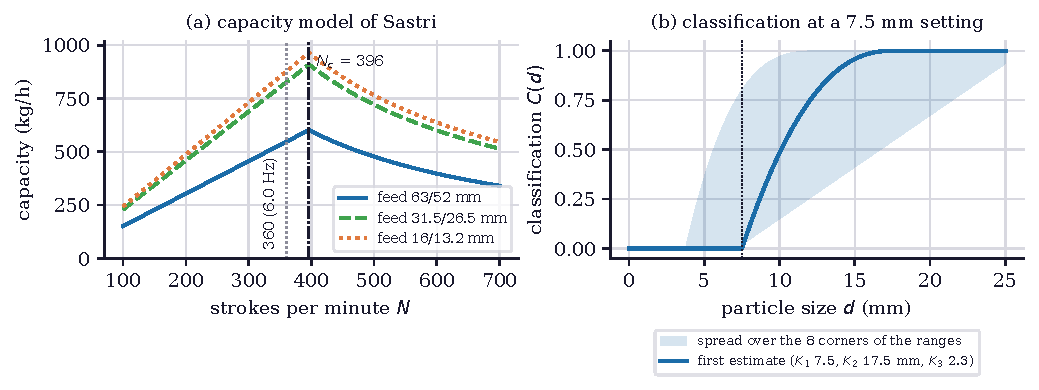
\includegraphics[width=\textwidth]{fig-labjaw.pdf}
\caption{The laboratory jaw of Barrios et al. in the population-balance evaluation, generated from the laboratory-jaw module. (a) Capacity of the jaw capacity model of Sastri against the stroke frequency for the three narrow feeds at a closed-side setting of $7.5$~mm, with the critical speed of Equation~\eqref{eq:sastri-nc} (dash-dot) and the operating speed of $360$ strokes per minute (dotted). (b) Classification of the first estimate (line) and the envelope of the eight corners of the ranges of King (shaded) at the same setting; the dotted line marks the setting. The figure shows the model before any comparison with a measurement.}
\label{fig:labjaw}
\end{figure}

\emph{The narrow feed class on the sieve grid.} A narrow feed class, such as $63/52$~mm, is the set of spheres whose diameters are uniform in $[d_{\mathrm l},d_{\mathrm u}]$ (lower and upper sieve of the class). The mass of a sphere goes as $d^3$, so the cumulative mass fraction passing $d$ goes as $d^4$ and the feed is known in closed form,
\begin{equation}
R_{\mathrm{cls}}(d)=\frac{d^4-d_{\mathrm l}^4}{d_{\mathrm u}^4-d_{\mathrm l}^4}\ \ (d_{\mathrm l}\le d\le d_{\mathrm u}),\qquad
F_{80}=\left[d_{\mathrm l}^4+0.8\left(d_{\mathrm u}^4-d_{\mathrm l}^4\right)\right]^{1/4},\qquad \bar F=\frac{d_{\mathrm l}+d_{\mathrm u}}{2},
\label{eq:labjaw-feed}
\end{equation}
integrated over each class of the sieve grid of Section~\ref{sec:notation} so that mass is conserved, with a sieve edge that equals a class limit up to the rounding of the grid giving no residue; the analytic $F_{80}$ is the one used for the reduction ratio, and $\bar F$, the arithmetic mean of the limits, is Sastri's average feed size (his Table 2 uses it). A class inside one sieve class gives one non-zero class. A feed class above the top of the grid, or with an upper limit at or above the gape, is refused.

\emph{Breakage and the Whiten solve.} The product is the engine's: the breakage function of Section~\ref{sec:m-breakage} with $t_{10}$ from the specific energy of the jaw, $E_{cs}=0.033\,T\,N/350$ (kWh/t, with the jaw's own throw $T$ in millimetres and $N$ in rpm), and the ore's $A\times b$, and the Whiten solve of Section~\ref{sec:m-whiten} with the classification of Equation~\eqref{eq:labjaw-first}. They are
reused and not repeated here. The solve returns the product mass per class, from which $P_{80}$ and $P_{50}$ are read by the grid's interpolation, and the reduction ratio is $F_{80}/P_{80}$ with the analytic $F_{80}$. The flags of the engine are kept in its own wording: a setting at or above the feed's lower limit is a pass-through regime, a reduction ratio below $1.05$ is negligible breakage, and an ill-conditioned breakage matrix
(a conditioning proxy above $10^{6}$) is flagged.

\emph{Bond's energy per unit of work index, and why no power is predicted.} Bond's third law gives the specific energy $W=10\,W_i\left(1/\sqrt{P_{80}}-1/\sqrt{F_{80}}\right)$ with the sizes in micrometres (Equation~\eqref{eq:bond}). The module returns the factor
\begin{equation}
w_{\mathrm B}=10\left(\frac{1}{\sqrt{P_{80}}}-\frac{1}{\sqrt{F_{80}}}\right)\quad[\mathrm{kWh/t\ per\ kWh/t\ of}\ W_i],\qquad W_i^{\ast}=\frac{E_{\mathrm m}}{w_{\mathrm B}},
\label{eq:labjaw-bond}
\end{equation}
the engine's Bond form at a work index of one, and the work index $W_i^{\ast}$ that a measured specific energy $E_{\mathrm m}$ (in kWh/t, $1$~kWh/t $=3600$~J/kg) would imply at the predicted sizes. No power is predicted, because no work index of the ore is published and the paper reports no Bond, JKMRC or drop-weight value for it; the implied work index states what the measured energy requires and is not a prediction. Bond's law has been compared with drawn power for plant jaws (the power efficiency of
the $36$ industrial jaws of $0.15$ to $1.68$~m gape of Sastri's Table 4 that have a drawn power ranges from $0.11$ to $3.26$~\cite{sastri1994}), and Donovan reports that for primary crushing the relevance of the law is questionable~\cite{donovan2003}; no test of it on a laboratory jaw was found, so a prediction would rest on an extrapolation without evidence. The net power of the paper was measured by an ammeter and may differ from a shaft power.

\emph{The link from the fracture energy to the ore's $A\times b$.} The engine needs the JKMRC product $A\times b$ of the ore, and the discrete element model has the fracture-energy parameters of Tavares. The two $t_{10}$ laws have the same exponential form, $t_{10}=A(1-e^{-bE_{cs}})$ (Equation~\eqref{eq:t10}, from the JKMRC~\cite{napier1996}) and $t_{10}=A\left(1-e^{-b'E/E_{50}}\right)$ (Equation~\eqref{eq:dem-t10}). Equating the exponents on one energy basis, with $1$~kWh/t $=3600$~J/kg,
\begin{equation}
b=\frac{3600\,b'}{E_{50}(d)},\qquad A\times b=\frac{3600\,A\,b'}{E_{50}(d)}\quad[\%\ \mathrm{per\ kWh/t}],
\label{eq:labjaw-axb}
\end{equation}
with $E_{50}$ in J/kg (Equation~\eqref{eq:dem-e50}), $A$ in percent and $b'$ dimensionless. No source states this conversion: it is the algebra of the two forms and is this work's, and the module (\texttt{axb\_from\_fracture\_energy}) says so. The two laws are equated with the ore's $A$ of $\demOreA$ percent, but the engine's \texttt{t10\_of} uses its own $A_{\mathrm e}=\demEngineA$ percent and $b=(A\times b)/A_{\mathrm e}$, so it evaluates the exponent of the link with another asymptote: at the coarse feed the engine's $t_{10}$ is $\demCoarseTtenEng$ percent against $\demCoarseTtenOreA$ percent with the ore's $A$ (the middle feed $\demMidTtenEng$ against $\demMidTtenOreA$, the fine feed $\demFineTtenEng$ against $\demFineTtenOreA$), a difference the evaluation does not correct. It carries a caveat: the size effect of $E_{50}(d)$ makes $b$ depend on the particle size, while the JKMRC fit and the engine hold $b$ constant for an ore, so the value is that of one size class; the
evaluation of a feed class takes the median fracture energy at the class's mean size, which is one reading of a quantity that the engine treats as a property of the ore. The link joins the two sides without a fit to the machine's results: both read the same single-particle fracture energies.

\begin{algorithm}[!t]
\caption{Evaluation of a narrow feed class on the laboratory jaw (\texttt{pipeline/\allowbreak{}model/\allowbreak{}crusher/\allowbreak{}labjaw.py}, \texttt{evaluate\_lab\_jaw} and \texttt{king\_band}).}
\label{alg:labjaw}
\begin{algorithmic}[1]
\Require jaw ($G$, $w$, $T$, $\rho_{\mathrm s}$, $k_{\mathrm M}$); class $[d_{\mathrm l},d_{\mathrm u}]$ with $d_{\mathrm u}<G$; setting $S$; speed $N$; ore $A\times b$; classification (default: Equation~\eqref{eq:labjaw-first})
\State $\mathbf f\gets$ the class on the sieve grid (Equation~\eqref{eq:labjaw-feed}); $F_{80}\gets$ its analytic value; $\bar F\gets(d_{\mathrm l}+d_{\mathrm u})/2$
\State $E_{cs}\gets0.033\,T\,N/350$; $t_{10}\gets\min\{0.44,\ A_{\mathrm e}(1-e^{-bE_{cs}})/100\}$ with $A_{\mathrm e}$ the engine's own $A$ and $b=(A\times b)/A_{\mathrm e}$; $\mathrm B\gets$ the breakage matrix; $\mathrm C\gets\mathrm{diag}(C(\bar d_k))$ of Equation~\eqref{eq:class}
\State $\mathbf p\gets$ the Whiten solution of Equation~\eqref{eq:whiten}; read $P_{80}$, $P_{50}$; $F_{80}/P_{80}$; flags
\State $D\gets$ Equation~\eqref{eq:sastri-d}; $N_c\gets$ Equation~\eqref{eq:sastri-nc}; $V_h\gets$ Equation~\eqref{eq:sastri-vh}; $Q_{\mathrm S}\gets$ Equation~\eqref{eq:sastri-q}
\State $w_{\mathrm B}\gets$ Equation~\eqref{eq:labjaw-bond}
\For{each of the eight corners $(\alpha_1,\alpha_2,K_3)$ of the ranges}
  \State repeat lines 2 and 3 with $K_1=\alpha_1S$, $K_2=\max(\alpha_2S,1.05K_1)$; keep the lowest and highest $P_{80}$, $P_{50}$ and passing at each sieve, with the corner
\EndFor
\State \Return the capacity with its factors, the product, the sizes, the reduction ratio, $w_{\mathrm B}$, the flags and the band
\end{algorithmic}
\end{algorithm}

\emph{Parameters.} The module's constants are those of the equations above, each a named constant with its unit: Sastri's $450$ (half the square of $30$~s per minute times the gravity's factor), $66.4$, $3.25$ and $1.15$, $0.21$ and $1.8$ with the gape switch at $0.25$~m, $0.85$ and $2.5$, $1.92$ and $6.5$; the first-estimate $K_3=2.3$; King's ranges; the engine's floor of $1.05$; Bond's $10$; and $3600$~J/kg per kWh/t. The laboratory jaw is the constants of the paper's Tables 2 and 3 (gape $90$~mm, width $140$~mm, throw $10$~mm, density $2.70$~t/m$^3$, $k_{\mathrm M}=1.0$); the closed-side setting and the stroke frequency are the operating point and not the machine.
The sources of each constant are in the module's comments and in the framework card of the method.

\emph{Complexity.} The capacity is a closed form of constant cost. The evaluation of a class costs one Whiten solve of the $K=28$ classes, $O(K^3)$ for the linear solve and $O(K^2)$ for the breakage matrix (Section~\ref{sec:m-whiten}), and the band costs eight of them; the whole evaluation of a feed class with its band is nine solves of a $28\times28$ system.

\emph{Implementation and tests.} The module is \texttt{data-pipeline/\allowbreak{}pipeline/\allowbreak{}model/\allowbreak{}crusher/\allowbreak{}labjaw.py}, standard library only and offline, with its tests in \texttt{tests/\allowbreak{}test\_labjaw.py}. The acceptance criteria that fail the build are: the nine rows of Table~\ref{tab:sastri} (eight within $0.2$ percent, the fifth within $3$ percent, stated); the values for the jaw of Barrios et al. to four significant figures; the capacity continuous at the critical speed
and at its peak there; the evaluation, the band and the ore link; and the refutations that no function of the module reads a measured throughput, power or product size and that the plant engine, the machine list and the learned models' encodings are untouched.
